\documentclass[11pt,a4paper]{article}
\usepackage[utf8]{inputenc}
\usepackage[T1]{fontenc}
\usepackage{amsmath,amssymb}
\usepackage{newtxtext,newtxmath}
\usepackage[margin=25mm]{geometry}
\usepackage{booktabs,graphicx,array,float}
\usepackage[table]{xcolor}
\usepackage{microtype}
\usepackage[section]{placeins}
\usepackage[hidelinks]{hyperref}
\setlength{\emergencystretch}{2em}
\renewcommand{\thesection}{S\arabic{section}}
\renewcommand{\thetable}{S\arabic{table}}
\renewcommand{\thefigure}{S\arabic{figure}}
\renewcommand{\theequation}{S\arabic{equation}}
\hypersetup{pdftitle={Supplementary material: Support-conditioned prediction combination for few-shot battery state-of-health estimation},pdfauthor={Zixuan Liu}}
\title{Supplementary material\\[5pt]\large Support-conditioned prediction combination for few-shot battery state-of-health estimation under operating-condition shift}
\author{Zixuan Liu}
\date{}
% Consistent fixed type size; never stretch tables to fill the column.
\newcommand{\papertablesize}{\fontsize{9}{11}\selectfont}

% Align dedicated float pages at the top with a fixed gap between floats.
\makeatletter
\setlength{\@fptop}{0pt}
\setlength{\@fpsep}{18pt}
\setlength{\@fpbot}{0pt plus 1fil}
\makeatother

% Prefer figures/tables accompanied by text over sparsely filled float pages.
\renewcommand{\topfraction}{.9}
\renewcommand{\bottomfraction}{.8}
\renewcommand{\textfraction}{.1}
\renewcommand{\floatpagefraction}{.8}

\begin{document}
\maketitle
This supplement presents selected design comparisons, effect-size analyses and reproducibility records for the frozen predictor reported in the main text. XJTU, MATR and Tongji remain development datasets. The seven-cell CALCE evaluation remains a frozen evaluation within a previously used public source, without overall MAE improvement. No model, training budget, eligibility rule or deployment weight was changed to prepare this supplement. Additional tables are generated from retained unrounded summaries; existing audit results are identified separately from new calculations on those summaries.

\section{Selected source-representation and expert-selection routes}
\label{sec:sdevelopment}
\subsection{M1 development alternatives}
Table~\ref{tab:sm1} selects ordinary GP enhancements and a PLS representation from the archived development screen. The pruned GP improves over the reported M1 on XJTU but performs worse on Tongji; ordinary PLS has lower MAE on XJTU and Tongji. Thus, the reported M1 is not a uniformly best standalone representation. Its main-text contribution includes representation learning and a source-selected adaptation mode, so the improvement cannot be attributed to representation alone. These routes document design alternatives and dataset-level trade-offs; they are not additional independent tests.

% Generated from unrounded frozen evidence by build_revision.py.
\begin{table}[H]\centering
\caption{Selected M1 development routes: aggregate MAE (SOH pp).}\label{tab:sm1}
\papertablesize\setlength{\tabcolsep}{4pt}\renewcommand{\arraystretch}{1.15}
\begin{tabular}{lrrr}\toprule
Route & XJTU & MATR & Tongji \\ \midrule
Original GPR & 3.0115 & 2.6862 & 6.6695 \\
Support posterior update & 3.0129 & 2.1955 & 6.8923 \\
Pruned GPR & 2.8989 & 2.3899 & 6.8422 \\
ARD GPR & 3.0241 & 2.6371 & 6.6927 \\
Group kernel & 5.4673 & 2.3968 & 5.5184 \\
Ordinary PLS metric & 2.8921 & 2.1884 & 5.1537 \\
Reported M1 (B1) & 2.9224 & 2.1837 & 5.3881 \\
\bottomrule\end{tabular}
\par\smallskip\begin{minipage}{\linewidth}\papertablesize All listed routes cover 55/180/130 cells. Earlier candidate metrics are stored as SOH ratios and are multiplied by 100 here. This is a selected development comparison, not a claim that the reported M1 dominates every alternative.\end{minipage}
\end{table}


\paragraph{Historical source-GPR diagnostic.}
The retained XJTU development diagnosis reports that all 3,577 query predictions in the 3C condition lie within 0.1 SOH pp of the source mean, approximately 99.077\%. The largest RBF correlation with any source sample is below 0.01, and current indicators account for 82.51\% of the summed standardized squared distances to nearest source samples. Distance shares are calculated by finding each query's nearest source point in the 21-indicator space, grouping squared coordinate differences by signal channel and summing across queries. This descriptive diagnostic does not establish a causal effect of current features. The same record identifies low-SOH overestimation in some conditions with closer source neighbours, so distance alone is not a complete explanation. Its query-pooled diagnostic errors must not replace the cell--domain aggregate errors of the main tables. The original report, including its historical hypotheses and subsequent-work proposals, is retained as \path{evidence/historical_gpr_diagnosis.md}; those proposals are not the definition of the final model.

\subsection{M2 reference-risk alternatives and frozen identity}
The reported M2 configuration is the frozen v3 candidate recorded in the selection manifest, with variant \texttt{source\_lodo\_reference\_bagged\_pca8}. Table~\ref{tab:sm2} compares fixed source LODO, HI-reference, unbagged PCA8-reference and bagged PCA8-reference candidates at the B12 stage. The unbagged candidate has lower XJTU MAE, fixed source LODO has the lowest MATR MAE in this comparison, and the frozen bagged candidate has lower Tongji MAE. These development outcomes document a trade-off rather than uniform dominance by v3.

% Generated from unrounded frozen evidence by build_revision.py.
\begin{table}[H]\centering
\caption{Selected M2 development candidates at the B12 stage: MAE (SOH pp).}\label{tab:sm2}
\papertablesize\setlength{\tabcolsep}{4pt}\renewcommand{\arraystretch}{1.15}
\begin{tabular}{lrrr}\toprule
Route & XJTU & MATR & Tongji \\ \midrule
Fixed source LODO & 2.7839 & 1.9274 & 3.4460 \\
HI reference risk (v1) & 2.7272 & 1.9405 & 3.4508 \\
Unbagged PCA8 reference risk (v2) & 2.6271 & 1.9950 & 3.4581 \\
Bagged PCA8 reference risk (v3, frozen) & 2.6567 & 1.9853 & 3.2965 \\
\bottomrule\end{tabular}
\par\smallskip\begin{minipage}{\linewidth}\papertablesize These are historical development candidates, not matched causal ablations of the final four-module model. The selection manifest identifies v3; no dataset-wise mixture of candidate versions is used.\end{minipage}
\end{table}


The fixed-source row uses the archived extended source-LODO configuration, without the later reference-risk aggregation. Its unrounded SOH-ratio metrics are converted to percentage points only when formatting Table~\ref{tab:sm2}.

The selection manifest records an explicit decision to retain v3. Earlier candidates are retained as development evidence; they are not substituted into individual dataset rows of B1234. This comparison changes historical candidate configurations and should not be interpreted as a matched causal ablation of bagging alone. The M3 selection manifest identifies \texttt{wave\_pair\_pca8\_global\_step\_0.5}, with the v3 M2 parent. Its candidate manifest and release-acceptance record are supplied separately; their hashes match the selection manifest. The unchanged M4 identity is the private-function candidate with global strength 0.5, recorded as \texttt{function\_private\_global\_step\_0.5}. Selection manifests and original candidate metrics are included in the evidence directory, with source paths and SHA-256 hashes in \path{evidence/provenance.json}.

\section{Paired and absolute waveform controls}
\label{sec:swaveform}
The M3 audit replaces paired PCA8 by absolute PCA8 while retaining the selected fold kernel, support-adaptation mode, latent dimension and gain. The paired input combines the current waveform and its difference from the early-support mean; the absolute control omits this pairing. These comparisons use the same permitted support and query information. The retained matched settings were selected for the paired candidate, so the matched comparison isolates the representation replacement at that operating point, not the best achievable result of each representation.

% Generated from unrounded frozen evidence by build_revision.py.
\begin{table}[H]\centering
\caption{Matched waveform comparison across all four M3 parent configurations. Each metric lists absolute (A) and paired (P) representations, in SOH pp.}\label{tab:sm3all}
\papertablesize\setlength{\tabcolsep}{4pt}\renewcommand{\arraystretch}{1.15}
\begin{tabular}{llrrrrrr}\toprule
Dataset & Output & MAE A & MAE P & RMSE A & RMSE P & P95 A & P95 P \\ \midrule
XJTU & B3 & 2.9349 & 2.9480 & 3.7046 & 3.7166 & 6.9644 & 6.9629 \\
XJTU & B13 & 2.8278 & 2.8325 & 3.5823 & 3.5723 & 6.8887 & 6.8041 \\
XJTU & B23 & 2.9109 & 2.9033 & 3.6396 & 3.6248 & 6.9560 & 6.8738 \\
XJTU & B123 & 2.6543 & 2.6459 & 3.3301 & 3.3067 & 6.3202 & 6.2701 \\
MATR & B3 & 2.5731 & 2.5715 & 3.4834 & 3.4661 & 6.9846 & 6.9091 \\
MATR & B13 & 2.1208 & 2.1041 & 3.0311 & 2.9979 & 6.4748 & 6.3772 \\
MATR & B23 & 2.1120 & 2.1172 & 2.8119 & 2.8137 & 5.6859 & 5.6628 \\
MATR & B123 & 1.9536 & 1.9514 & 2.6381 & 2.6258 & 5.4424 & 5.3850 \\
Tongji & B3 & 6.0807 & 5.8459 & 7.4688 & 7.2338 & 13.6144 & 13.3477 \\
Tongji & B13 & 5.0776 & 4.9346 & 6.1062 & 5.9624 & 10.5181 & 10.3128 \\
Tongji & B23 & 3.3679 & 3.3151 & 4.1703 & 4.0763 & 7.0561 & 6.8063 \\
Tongji & B123 & 3.1560 & 3.0783 & 3.9502 & 3.8408 & 6.7214 & 6.4840 \\
\bottomrule\end{tabular}
\end{table}


Table~\ref{tab:sm3all} retains all four M3 parent configurations. In B123, pairing improves MAE, RMSE and P95 on all three datasets. Other configurations contain exceptions: for example, the absolute representation has lower XJTU MAE in B3 and B13, and lower MATR MAE in B23. The full results therefore support a configuration-dependent benefit rather than universal necessity.

Table~\ref{tab:sm3selected} provides the complementary comparison in which each representation uses its own source-validation-selected configuration, followed by the same global multiplier 0.5. The absolute representation has lower MATR MAE, RMSE and P95, while the paired representation has lower errors on XJTU and Tongji. These settings remain exploratory development choices. Both comparison types are reported without selecting a dataset-specific winner for the final predictor.

% Generated from unrounded frozen evidence by build_revision.py.
\begin{table}[H]\centering
\caption{B123 waveform alternatives with separate source-validation selection and common global strength 0.5. Errors are SOH pp.}\label{tab:sm3selected}
\papertablesize\setlength{\tabcolsep}{4pt}\renewcommand{\arraystretch}{1.15}
\begin{tabular}{llrrr}\toprule
Dataset & Representation & MAE & RMSE & P95 \\ \midrule
XJTU & Absolute & 2.6697 & 3.3695 & 6.4125 \\
XJTU & Paired & 2.6459 & 3.3067 & 6.2701 \\
MATR & Absolute & 1.9381 & 2.5990 & 5.3265 \\
MATR & Paired & 1.9514 & 2.6258 & 5.3850 \\
Tongji & Absolute & 3.3600 & 4.1358 & 6.9964 \\
Tongji & Paired & 3.0783 & 3.8408 & 6.4840 \\
\bottomrule\end{tabular}
\end{table}


\section{Module effect sizes and paired uncertainty}
\label{sec:seffects}
Let $m(A)$ be the dataset-level MAE of the base predictor with module subset $A\subseteq\{1,2,3,4\}$, using the main-text cell--domain weighting. Three summaries answer different questions:
\begin{align}
\text{Progressive increment:}\quad
\Delta_m^{\mathrm{prog}}&=m(\{1,\ldots,m\})-m(\{1,\ldots,m-1\}),\\
\text{Leave-one-module-out loss:}\quad
L_m&=m(\{1,2,3,4\}\setminus\{m\})-m(\{1,2,3,4\}),\\
\text{Average marginal effect:}\quad
\overline\Delta_m&=\frac{1}{8}\sum_{A\subseteq\{1,2,3,4\}\setminus\{m\}}
\big[m(A\cup\{m\})-m(A)\big].
\end{align}
The empty subset denotes B. Progressive increments and average marginal effects are error changes, so negative values favour adding the module. Leave-one-module-out loss is positive when removing the module worsens the full model. These summaries depend on their parent configurations and must not be added together or interpreted as independent causal contributions. The eight parent configurations are not eight independent experiments.

% Generated from unrounded frozen evidence by build_revision.py.
\begin{table}[H]\centering
\caption{Three distinct summaries of module effects on MAE (SOH pp).}\label{tab:seffects}
\papertablesize\setlength{\tabcolsep}{4pt}\renewcommand{\arraystretch}{1.15}
\begin{tabular}{llrrr}\toprule
Dataset & Module & Progressive & Leave-one-out & Average marginal \\ \midrule
XJTU & M1 & -0.0891 & 0.2537 & -0.1924 \\
XJTU & M2 & -0.2657 & 0.1638 & -0.1406 \\
XJTU & M3 & -0.0108 & 0.0027 & -0.0461 \\
XJTU & M4 & -0.0083 & 0.0083 & -0.0166 \\
MATR & M1 & -0.5025 & 0.1593 & -0.3204 \\
MATR & M2 & -0.1984 & 0.1436 & -0.3234 \\
MATR & M3 & -0.0339 & 0.0268 & -0.0634 \\
MATR & M4 & -0.0315 & 0.0315 & -0.0478 \\
Tongji & M1 & -1.2813 & 0.1856 & -0.6403 \\
Tongji & M2 & -2.0916 & 1.5118 & -2.1921 \\
Tongji & M3 & -0.2183 & 0.1635 & -0.4006 \\
Tongji & M4 & -0.2275 & 0.2275 & -0.4792 \\
\bottomrule\end{tabular}
\par\smallskip\begin{minipage}{\linewidth}\papertablesize Progressive increments and average marginal effects are new minus parent error (negative favours addition). Leave-one-module-out loss is error without the module minus full-model error (positive favours retention). The columns are alternative summaries and are not additive independent causal contributions.\end{minipage}
\end{table}


The full sixteen-configuration, three-metric table is retained in the main text and as \path{evidence/aggregate.csv}. Table~\ref{tab:seffects} derives its three summaries from those unrounded entries. It shows much larger M1/M2 than M3/M4 leave-one-out losses on XJTU and MATR, and a particularly large M2 loss on Tongji. The sign of all aggregate additions alone does not establish equal necessity or equal effect size.


% Generated from unrounded frozen evidence by build_revision.py.
\begin{table}[!htbp]\centering
\caption{Progressive MAE increments and 95\% domain-bootstrap intervals (SOH pp). Negative changes favour the added branch.}\label{tab:branchintervals}
\papertablesize\setlength{\tabcolsep}{4pt}\renewcommand{\arraystretch}{1.15}
\begin{tabular}{lrrrr}\toprule
Dataset & $\Delta_3$ & 95\% interval & $\Delta_4$ & 95\% interval \\ \midrule
XJTU & -0.0108 & [-0.1150, 0.1065] & -0.0083 & [-0.0340, 0.0146] \\
MATR & -0.0339 & [-0.1261, 0.0465] & -0.0315 & [-0.0977, 0.0033] \\
Tongji & -0.2183 & [-0.3688, -0.0688] & -0.2275 & [-0.3372, -0.1244] \\
\bottomrule\end{tabular}
\par\smallskip\begin{minipage}{\linewidth}\papertablesize $\Delta_3=\mathrm{MAE}_{B123}-\mathrm{MAE}_{B12}$ and $\Delta_4=\mathrm{MAE}_{B1234}-\mathrm{MAE}_{B123}$. The 5,000 whole-domain resamples concern fixed selected predictions, not repeated training, and do not correct for development selection.\end{minipage}
\end{table}


Table~\ref{tab:branchintervals} gives the retained progressive M3/M4 intervals, with 5,000 whole-domain resamples and seed 91010. The resampling preserves cells within each selected domain; there are only 6, 4 and 11 domains. Both Tongji intervals lie below zero, whereas both intervals on XJTU and MATR cross zero. These intervals measure variation of fixed selected predictions over observed domains, not full-training variability, and do not correct for architecture or global-strength selection. Crossing zero does not prove absence of an effect.

For the reported complete predictor, the M4 source-selected gain is zero in five folds: XJTU 3C, R3 and R2.5, and MATR b2 and b4. They contain 119 cells. B1234 therefore equals B123 on those folds by the selected zero-weight setting; M4 is not an active adjustment for every target cell. Figure~\ref{fig:sdomains} shows the progressive reductions for all 21 held-out groups. Its positive reduction convention is the negative of the progressive error-change convention above.
\begin{figure}[!htbp]\centering
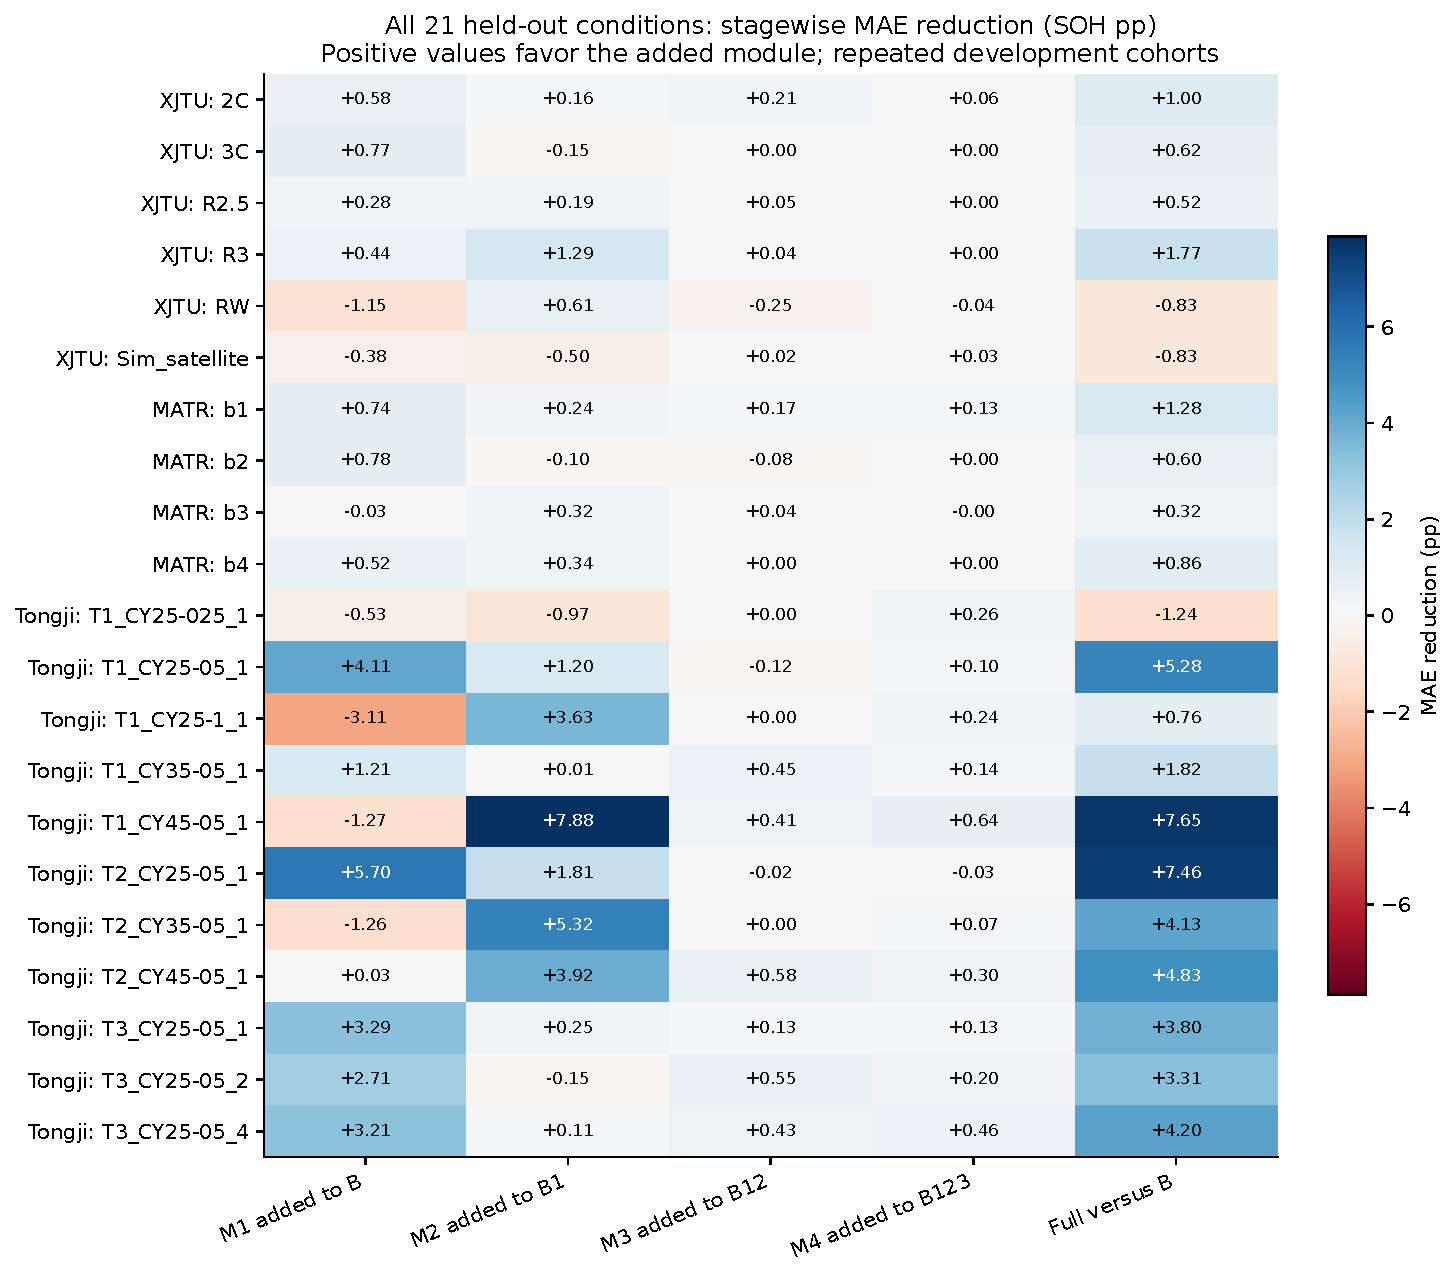
\includegraphics[width=.96\linewidth,height=.76\textheight,keepaspectratio]{figures_revision/domain_effects.pdf}
\caption{All 21 development groups. Values are parent MAE minus new-stage MAE (SOH pp), so positive values favour the added module. The final column is B minus B1234. These are repeated development cohorts; the entries are not independent confirmatory trials.}\label{fig:sdomains}
\end{figure}

\section{Optimization sensitivity and reproducibility scope}
\label{sec:saudit}
\subsection{Source-GP initialization and risk resampling}
The retained source-GP experiment evaluates length-scale initialization multipliers 0.5, 0.8, 1.0, 1.25 and 2.0 relative to the original prior across the 21 outer folds. The 105 fixed-branch source fits include the audited pilot fold reused by the batch; all five outcomes per fold are retained instead of selecting the best initialization. The representation, label budget, selected kernel, blend strength, target mode and outer selections remain fixed. Table~\ref{tab:sinit} shows the complete-model MAE for each initialization.

% Generated from unrounded frozen evidence by build_revision.py.
\begin{table}[H]\centering
\caption{Complete-model MAE under five source-GP length-scale initialization multipliers (SOH pp).}\label{tab:sinit}
\papertablesize\setlength{\tabcolsep}{4pt}\renewcommand{\arraystretch}{1.15}
\begin{tabular}{lrrr}\toprule
Initial multiplier & XJTU & MATR & Tongji \\ \midrule
0.5 & 2.637574504 & 1.919921656 & 2.850804583 \\
0.8 & 2.637574475 & 1.919921589 & 2.850807527 \\
1.0 & 2.637574820 & 1.919921668 & 2.850807583 \\
1.25 & 2.637574499 & 1.919921613 & 2.850805801 \\
2.0 & 2.637574526 & 1.919921644 & 2.850804445 \\
\bottomrule\end{tabular}
\par\smallskip\begin{minipage}{\linewidth}\papertablesize Multipliers apply to the original prior length scale. Extra digits show numerical sensitivity, not measurement precision. Representation, selected kernel, label budget, blend strength and target mode remain fixed; all five outcomes are retained.\end{minipage}
\end{table}


The maximum-minus-minimum MAE ranges are approximately $3.45\times10^{-7}$, $7.85\times10^{-8}$ and $3.14\times10^{-6}$ pp for XJTU, MATR and Tongji. The archived screen retains all 32 module-addition checks under all five initializations. This supports numerical stability with respect to the tested source-GP initialization; it is not five complete pipeline random-seed repetitions. Preparing this supplement reuses those fitted results and does not refit the GPs. The prior asset audit also records that the signal-amplitude parameter reaches its bound for all five initializations in the Tongji1\_CY25-1\_1 fold. Consequently, numerical agreement of final predictions does not establish an unconstrained optimum or the absence of fitting-boundary issues.

The separate ten-draw risk-resampling analysis retains the fitted GPs and changes reference-risk weights. All eight M4 additions pass the three-dataset, three-metric checks in all ten draws; all 32 additions pass in eight draws, with remaining failures involving M2. Risk resampling and source-GP initialization probe different sources of sensitivity. Neither repeats the full architecture-selection process.

\subsection{Leave-one-dataset-out selection audit}
The main text reports a sensitivity analysis for the fact that XJTU, MATR and Tongji informed architecture and global-strength selection. The audit contains 35 frozen candidates, formed by seven architecture families crossed with five global steps. In each of three rounds, one complete dataset is excluded from candidate selection; the other two datasets select the candidate and global step, which are then evaluated on the held-out dataset. The selected candidates are plain/1.0 for XJTU, condition\_mixed/1.0 for MATR and plain/0.5 for Tongji. Their LODO MAEs are 2.6855, 2.0178 and 2.9666 pp, versus base-GPR MAEs of 3.0115, 2.6862 and 6.6695 pp. The corresponding relative reductions are 10.83\%, 24.89\% and 55.52\%.

\begin{table}[!htbp]
\centering
\caption{Leave-one-dataset-out selection-level audit. Each held-out dataset is excluded from candidate selection; the other two development datasets select among 35 frozen candidates (seven architecture families by five global steps).}
\label{tab:lodo}
\scriptsize
\setlength{\tabcolsep}{4pt}
\begin{tabular}{lccrr}
\toprule
Held-out dataset & Selected candidate & Global step & LODO MAE & Base GPR MAE \\
\midrule
XJTU & plain & 1.0 & 2.6855 & 3.0115 \\
MATR & condition\_mixed & 1.0 & 2.0178 & 2.6862 \\
Tongji & plain & 0.5 & 2.9666 & 6.6695 \\
\bottomrule
\end{tabular}
\begin{flushleft}
\scriptsize Relative reductions are 10.83\%, 24.89\% and 55.52\%, respectively. This is a frozen-candidate selection-level audit, not complete nested cross-validation with retraining from raw data.
\end{flushleft}
\end{table}


This result indicates that the relative advantage does not disappear when the dataset used for evaluation is excluded from candidate selection. The scope must be stated precisely: the audit reuses frozen candidate outputs and probes selection sensitivity at the dataset level; it is not a complete nested cross-validation that retrains every architecture from raw data within each outer loop. The original run report, candidate results, selection records and verification record are identified in \path{evidence/lodo_selection_audit.md} and the accompanying experiment archive.

\subsection{Neural training records and checkpoint replay}
The neural comparison comprises three methods, 21 folds and three seeds, giving 189 source-training task records. The supplemental baseline study reused 54 verified XJTU source checkpoints and generated the remaining 135 MATR/Tongji source-checkpoint fits, together with the source-validation candidate fits. The retained audit reports validation-patience stopping for all 189 tasks; it does not establish that all architecture families received identical optimization effort.

% Generated from unrounded frozen evidence by build_revision.py.
\begin{table}[H]\centering
\caption{Scope and numerical differences in the retained neural checkpoint audit.}\label{tab:sneural}
\papertablesize\setlength{\tabcolsep}{4pt}\renewcommand{\arraystretch}{1.15}
\begin{tabular}{ll}\toprule
Check & Coverage / maximum difference \\ \midrule
Source-validation task scores & 189 \\
Primary cell--seed predictions & 3,285 \\
Cell--seed--setting predictions & 9,855 \\
Applicable support-fit-state replays & 93 \\
Source-validation score difference & $3.17\times10^{-9}$ SOH ratio \\
Saved-prediction replay difference & $4.77\times10^{-7}$ SOH ratio \\
Current-query numerical difference & $1.73\times10^{-6}$ SOH ratio \\
\bottomrule\end{tabular}
\par\smallskip\begin{minipage}{\linewidth}\papertablesize Differences are in normalized SOH units, not percentage points; multiply by 100 for pp. The saved-prediction maximum is therefore approximately $4.77\times10^{-5}$ pp. Counts describe distinct audit operations and must not be added as independent experiments.\end{minipage}
\end{table}


The 3,285 primary cell--seed predictions correspond to 365 cells, three methods and three seeds. Three evaluated settings (source-selected, source-only and support-bias-corrected) give 9,855 cell--seed--setting predictions. Applicable support-fit-state reconstruction was checked in 93 cases using early support, not in every cell. Source-validation score replay, saved-prediction replay and current-query checks are separate operations with separate numerical tolerances. Replaying a saved source checkpoint does not retrain it.

The nine historical reference/classical families do not have equivalent per-query and checkpoint-replay coverage. Their retained cell metrics can be reaggregated, but the neural replay counts cannot be extended to those families. Numerical agreement supports reproduction of the recorded local implementations; it does not establish equal search budgets, globally optimal training or faithful reproduction of every published architecture.

\subsection{Historical baseline coverage}
The earlier XJTU screen contains 19 strict-track method families, whereas the main three-dataset table contains 12. The seven additional neural families are MLP, CNN1D, LSTM, GRU, CNN--LSTM, Transformer and PatchTST-CI-SOH. Their retained results cover XJTU only; they were not extended to MATR and Tongji in the supplemental baseline study. The historical screen also contains separate cycle-information routes, whose additional inputs prevent pooling them with the strict waveform comparison.

The original historical comparison and the subsequent coverage report are retained in \path{evidence/historical_xjtu_comparison.md} and \path{evidence/historical_baseline_scope.md}. Their setting and seed counts describe those historical runs, not the current source-selected three-dataset comparison. We retain adverse results and incomplete coverage without selecting the best historical setting to replace a primary-table entry. The 189-task neural replay audit above applies to its three stated methods, not to all 19 historical families.

\subsection{Frozen-model acceptance and information-boundary scope}
The retained M4 acceptance record covers 21 folds, 365 cells, 168 adapters and 5,840 cell--configuration metric rows. It explicitly distinguishes exported-model boundary probes on one cell per fold from separately audited branch boundary checks on all 365 cells. The record links metric verification, runtime replay and snapshot checks by hashes; these cover different operations and are not interchangeable. \path{evidence/m4_acceptance.json} records this scope and the final experimental release. Reading that acceptance record for this revision does not repeat its historical checks. The early-label and future-signal restrictions tested by such probes concern information access, not robustness to measurement noise or missing charge windows.

\subsection{What each verification establishes}
\begin{itemize}
\item \textbf{Metric recalculation} reads saved labels and predictions and reconstructs errors. The existing asset audit reports agreement for 5,840 development cell--configuration rows and all 210 CALCE stage/source/cell prediction files. This is not an inference replay.
\item \textbf{Inference replay} loads a saved checkpoint or adapter and recomputes predictions. The neural scope is given in Table~\ref{tab:sneural}; source training is not repeated.
\item \textbf{Source-GP initialization sensitivity} reuses the results of fitting the fixed branch from five starting length scales. It does not vary the complete pipeline.
\item \textbf{Domain bootstrap} resamples whole observed domains for fixed predictions. It does not remove development-selection bias.
\item \textbf{Risk resampling} changes empirical reference-risk draws with fitted GPs held fixed. It is not a substitute for training-seed or measurement-noise experiments.
\end{itemize}
Different support budgets, label and signal noise, missing charge windows, full-pipeline retraining, calibrated predictive intervals and independent acquisition sources remain outside these verification claims.

\section{CALCE protocol and trajectory diagnostics}
\label{sec:scalce}
This section reports the detailed frozen XJTU-to-CALCE boundary analysis omitted from the main text. The purpose is to assess transfer under a different acquisition source and protocol while keeping the source models, model identity and deployment weights fixed. CALCE measurements are available from the Center for Advanced Life Cycle Engineering battery archive at \url{https://web.calce.umd.edu/batteries/data/}.
\subsection{Frozen evaluation protocol}
The frozen XJTU models were applied to fourteen candidate cells: CS2\_5/6/7/8/21/24/25, CX2\_3/4/31 and PL11--PL14. Seven met the input and capacity requirements: CS2\_5, CS2\_6, CX2\_3 and PL11--PL14. They provide 5,633 eligible measurement pairs, consisting of 70 support and 5,563 query pairs.

Eligibility requires a 3.9--4.1 V charge segment, an interpretable full-discharge capacity and more than ten eligible pairs in chronological order. CS2\_7 fails the complete-window/discharge checks; CS2\_24 and CS2\_25 supply only one and two qualified pairs, respectively. For CS2\_8/21 and CX2\_4/31, the interpretation of capacity units and chronology remains unresolved. Two unverified TXT records within CX2\_3 are excluded at the file level. Exclusions are based on measurement interpretation and availability, not model error.

The complete-charge gate requires at least 4.18 V. The CS2/CX2 full-reference discharge gate uses an under-load voltage at or below 2.72 V; PL follows its 2.75-V cutoff with a 0.02-V tolerance. Capacity is based on full-discharge counter increments checked against current integrals. Missing labels are not interpolated. The first ten eligible reference measurements need not be the first ten physical ageing cycles, and labels remain discharge-rate-specific.

The seven cells form four protocol groups: CS2 low-SOC-ageing reference tests, CX2 alternating-pulse full references, PL full-SOC 0.5C discharge and PL full-SOC 2C discharge. All six XJTU source-fold models are evaluated separately; errors are averaged over source models, equally over cells within a group and then equally over the four groups. Predictions are not ensembled, and the six source models do not create 42 independent target cells. Source models, blend weights and the complete-model identity are fixed before this evaluation. Local records contain no earlier model scores for the seven selected cells, although other CALCE cells had been used in the project.

% Original numerical entries retained; cohort and cell results presented together.
\begin{table}[!p]\renewcommand{\arraystretch}{1.15}\centering
\caption{Frozen XJTU-to-CALCE evaluation. Errors are SOH pp.}\label{tab:calcemain}
\papertablesize\setlength{\tabcolsep}{3pt}
\textit{A. Equal protocol-group and source-model weighting}\\[4pt]
\begin{tabular}{lrrr}
\toprule
Configuration & MAE & RMSE & P95 \\
\midrule
B & 13.7358 & 16.3646 & 29.8797 \\
B1 & 13.8244 & 16.4608 & 30.0304 \\
B12 & 13.8535 & 16.4864 & 30.0643 \\
B123 & 13.7812 & 16.4215 & 29.9881 \\
B1234 & 13.7817 & 16.4220 & 29.9888 \\
\bottomrule
\end{tabular}
\par\medskip
\textit{B. Cell MAE averaged over six frozen source models}\\[4pt]
\begin{tabular}{lrccccc}
\toprule
Cell & Queries & B & B1 & B12 & B123 & B1234 \\
\midrule
CS2\_5 & 59 & 3.4475 & 3.7040 & 3.5342 & 3.4869 & 3.4953 \\
CS2\_6 & 55 & 15.5305 & 14.7379 & 14.2676 & 14.2248 & 14.2343 \\
CX2\_3 & 1750 & 24.6673 & 24.2247 & 24.1338 & 24.0111 & 24.0156 \\
PL11 & 870 & 9.3276 & 9.1544 & 8.8574 & 8.7604 & 8.7725 \\
PL12 & 972 & 15.6624 & 17.9360 & 19.4745 & 19.4378 & 19.3949 \\
PL13 & 871 & 8.3137 & 8.2983 & 8.0672 & 7.9676 & 7.9762 \\
PL14 & 986 & 8.2699 & 8.3152 & 8.3592 & 8.3500 & 8.3494 \\
\bottomrule
\end{tabular}
\par\smallskip\begin{minipage}{\columnwidth}\papertablesize Every cell supplies ten support measurements in addition to the listed queries. Source models are scored separately; predictions are not ensembled. Panel A weights four protocol groups equally, rather than taking a direct average of the seven cell rows.\end{minipage}
\par\vspace{16pt}
\caption{CALCE protocol-group decomposition of MAE (SOH pp).}\label{tab:calceprotocols}
\papertablesize\setlength{\tabcolsep}{4pt}\renewcommand{\arraystretch}{1.15}
\begin{tabular}{lrrrr}\toprule
Protocol group & Cells & B & B1234 & $\Delta$ \\ \midrule
CS2 low-SOC RPT & 2 & 9.4890 & 8.8648 & -0.6242 \\
CX2 alternating pulse & 1 & 24.6673 & 24.0156 & -0.6517 \\
PL full-SOC 0.5C discharge & 2 & 8.8206 & 8.3744 & -0.4462 \\
PL full-SOC 2C discharge & 2 & 11.9661 & 13.8721 & +1.9060 \\
Equal protocol mean & 7 & 13.7358 & 13.7817 & +0.0460 \\
\bottomrule\end{tabular}
\par\smallskip\begin{minipage}{\linewidth}\papertablesize $\Delta=\mathrm{MAE}_{B1234}-\mathrm{MAE}_B$. Errors are averaged over six separately scored source models, equally over cells within each group and then equally over the four groups. Protocol differences do not isolate a causal discharge-rate effect.\end{minipage}

\end{table}


\subsection{Protocol-dependent error changes}
Table~\ref{tab:calceprotocols} separates CS2 low-SOC RPT, CX2 alternating-pulse full references, PL full-SOC 0.5C discharge and PL full-SOC 2C discharge. Three groups improve, while the last worsens by 1.9060 pp. Equal protocol weighting yields a $+0.0460$-pp MAE difference, as illustrated in Figure~\ref{fig:scalceprotocol}. Protocol, cell population and capacity definition are confounded, so this comparison does not identify a causal discharge-rate effect. The four protocol groups are not a controlled rate experiment.
\begin{figure}[!htbp]\centering
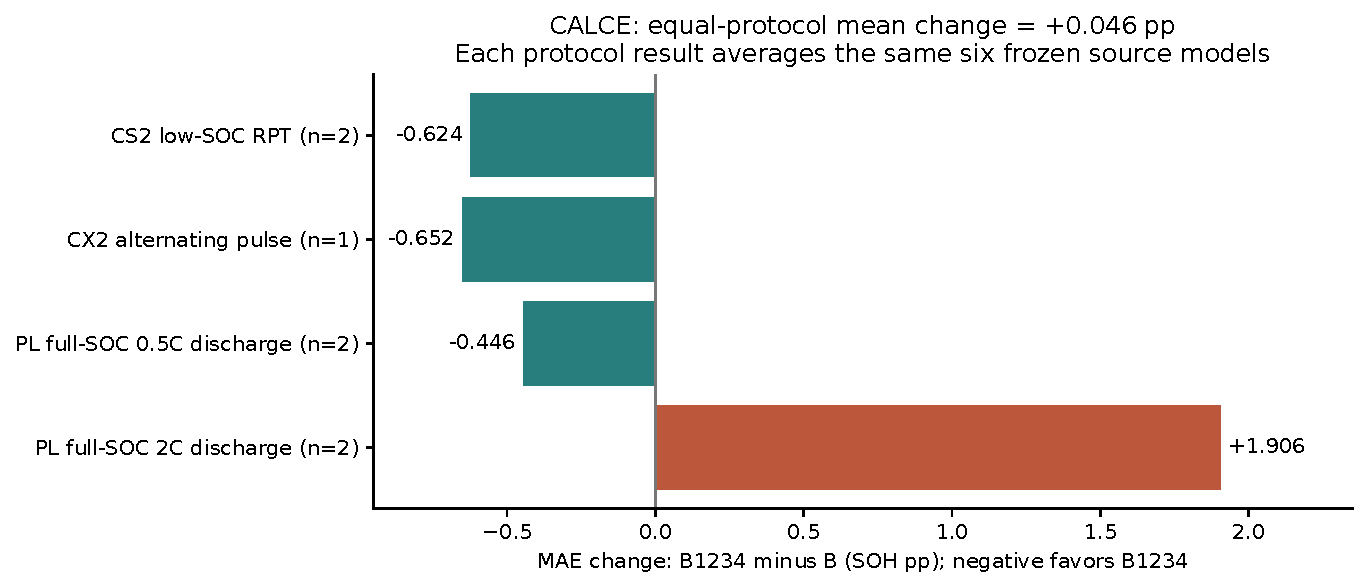
\includegraphics[width=\linewidth]{figures_revision/calce_protocols.pdf}
\caption{Protocol-group MAE changes for B1234 relative to B. Errors are averaged over six separately scored frozen source models and equally over cells within each protocol group. Bars are descriptive means, not confidence intervals.}\label{fig:scalceprotocol}
\end{figure}

\subsection{Prediction-range definition and all-cell results}
For each frozen source fold and eligible CALCE cell, the prediction range is computed over the same query interval used for the error metrics:
\begin{equation}
R_{fc}^{\mathrm{pred}}=100\left(\max_{j>K}\widehat y_{fcj}-\min_{j>K}\widehat y_{fcj}\right),\qquad
R_c^{\mathrm{obs}}=100\left(\max_{j>K}y_{cj}-\min_{j>K}y_{cj}\right).
\end{equation}
The base-GPR trajectories have zero range in all 42 saved source-fold/cell arrays. For B1234, the overall maximum is the maximum of $R_{fc}^{\mathrm{pred}}$ over six source folds and seven cells, without averaging predictions into a new ensemble. Table~\ref{tab:sranges} shows the minimum and maximum over source models for each cell. The largest B1234 range is 1.9427 pp, whereas observed query ranges span 5.4231--70.8928 pp.

% Generated from unrounded frozen evidence by build_revision.py.
\begin{table}[H]\centering
\caption{CALCE query SOH ranges (percentage points).}\label{tab:sranges}
\papertablesize\setlength{\tabcolsep}{4pt}\renewcommand{\arraystretch}{1.15}
\begin{tabular}{lrrr}\toprule
Cell & Observed range & Min. B1234 range & Max. B1234 range \\ \midrule
CS2\_5 & 5.4231 & 0.0471 & 1.4674 \\
CS2\_6 & 35.4190 & 0.0404 & 1.1624 \\
CX2\_3 & 60.3571 & 0.0275 & 1.1215 \\
PL11 & 21.9470 & 0.0107 & 0.7986 \\
PL12 & 70.8928 & 0.0321 & 1.6130 \\
PL13 & 20.8451 & 0.0081 & 0.9452 \\
PL14 & 56.1903 & 0.0593 & 1.9427 \\
\bottomrule\end{tabular}
\par\smallskip\begin{minipage}{\linewidth}\papertablesize Each source-fold/cell range is computed on the query interval used for its error metrics. Minima and maxima are over six individual source-model predictions per cell; no ensemble is formed. B has zero range in all 42 saved arrays.\end{minipage}
\end{table}


Figure~\ref{fig:scalcetrajectories} retains all seven eligible cells and plots each source model separately. The complete predictor introduces nonzero variation but does not recover the observed external capacity-change amplitude. Some cell-level MAE reductions therefore cannot be taken as evidence of successful degradation tracking. These are diagnostics of stored output behaviour; they do not establish a unique kernel-distance, representation or physical failure mechanism.
\begin{figure}[!htbp]\centering
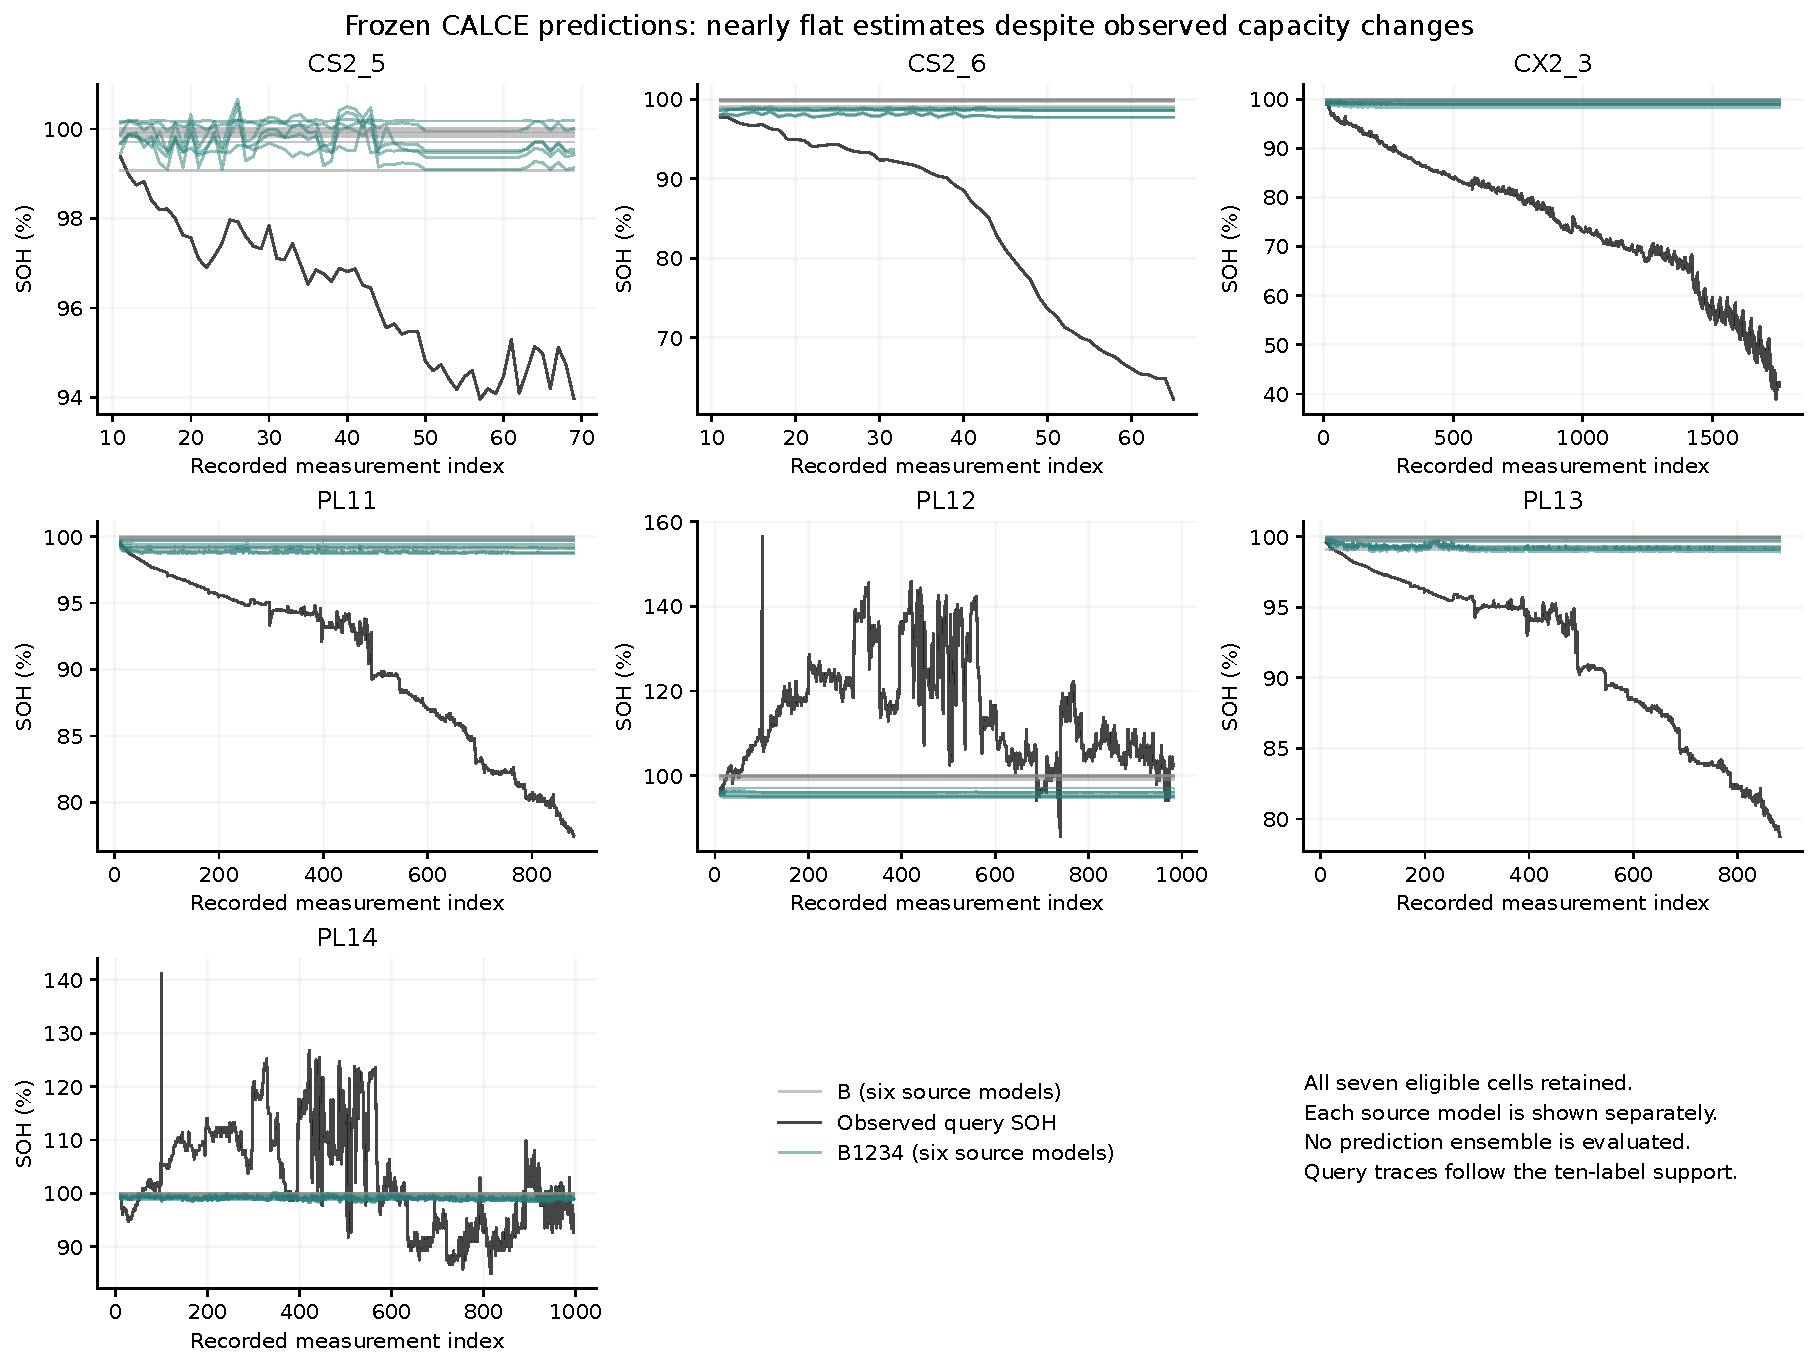
\includegraphics[width=\linewidth,height=.78\textheight,keepaspectratio]{figures_revision/calce_trajectories.pdf}
\caption{Observed query SOH and saved B/B1234 predictions for all seven eligible CALCE cells. Each of the six frozen XJTU source models is plotted separately; overlapping lines may be indistinguishable. Measurement indices are display axes, not model inputs. No prediction ensemble is evaluated.}\label{fig:scalcetrajectories}
\end{figure}

\section{Accuracy--cost operating points and evidence provenance}
\label{sec:scost}
\subsection{Measured operating points}
Table~\ref{tab:scost} relates B12 and B1234 to their shared baseline B. B12 retains most of the aggregate reduction, while additional conditioning achieves lower complete-model errors at additional query cost. Figure~\ref{fig:scost} places all five measured stages on the same accuracy--latency axes. These are fixed operating points, not a new target-adaptive stage selector; no stage is retrospectively selected for each held-out group. Timings describe the specified CPU implementation and exclude signal acquisition and capacity-label measurement.

% Generated from unrounded frozen evidence by build_revision.py.
\begin{table}[H]\centering
\caption{B12 and complete-model operating points. MAE is in SOH pp and latency in ms.}\label{tab:scost}
\papertablesize\setlength{\tabcolsep}{4pt}\renewcommand{\arraystretch}{1.15}
\begin{tabular}{lrrrrr}\toprule
Dataset & B12 MAE & Full MAE & Gain retained & B12 ms & Full ms \\ \midrule
XJTU & 2.6567 & 2.6376 & 94.9\% & 8.79 & 15.40 \\
MATR & 1.9853 & 1.9199 & 91.5\% & 5.77 & 8.83 \\
Tongji & 3.2965 & 2.8508 & 88.3\% & 6.78 & 14.26 \\
\bottomrule\end{tabular}
\par\smallskip\begin{minipage}{\linewidth}\papertablesize Gain retained is $100(\mathrm{MAE}_B-\mathrm{MAE}_{B12})/(\mathrm{MAE}_B-\mathrm{MAE}_{B1234})$. It is neither an accuracy percentage nor an equivalence test.\end{minipage}
\end{table}


\begin{figure}[!htbp]\centering
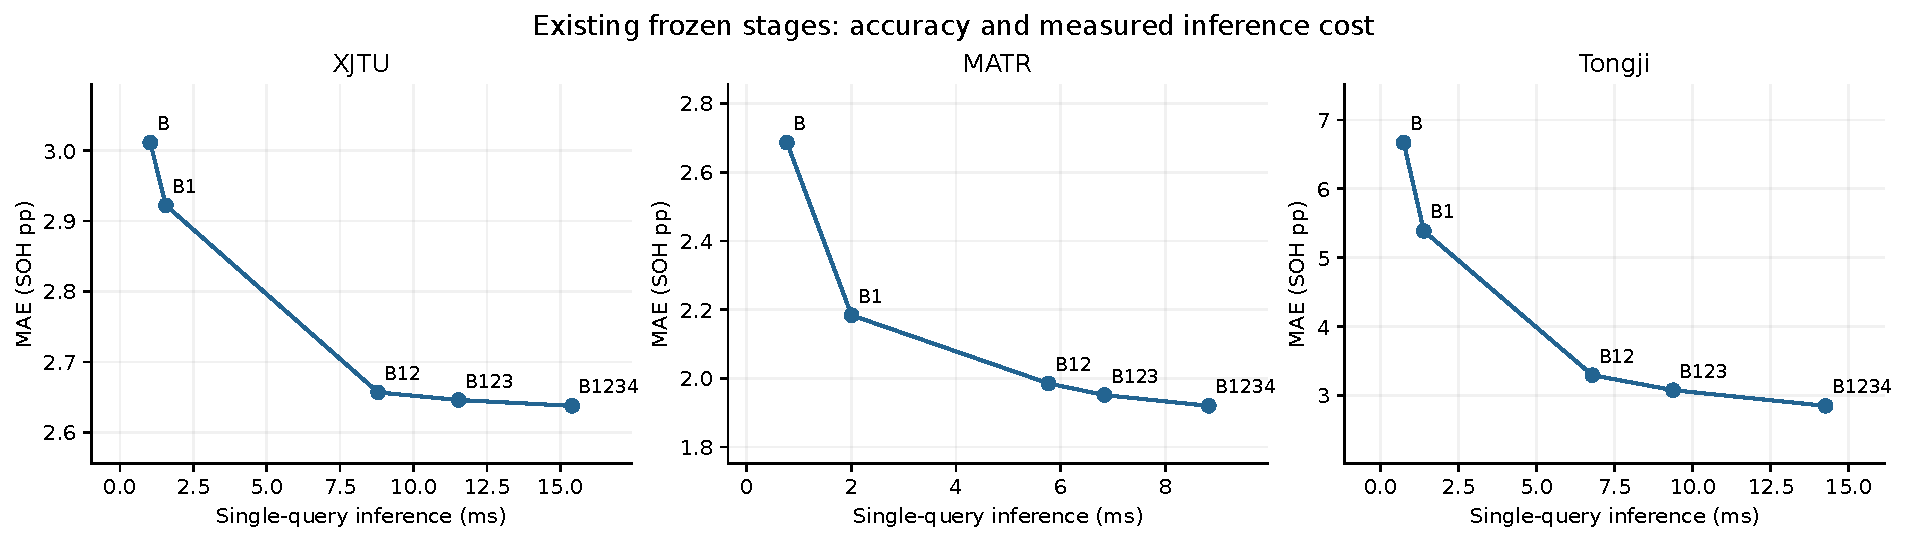
\includegraphics[width=\linewidth]{figures_revision/stage_cost.pdf}
\caption{Aggregate MAE and measured single-query CPU time for B, B1, B12, B123 and B1234. The stages reuse the existing timing protocol; connecting lines indicate the progressive construction order, not a continuous fitted trade-off curve.}\label{fig:scost}
\end{figure}

\subsection{Source records, hashes and reproduction boundary}
The prior asset audit reports 129,192 files and 77,110,506,591 bytes, with streamed file hashing and type-specific parsing. This revision uses that retained audit and targeted source checks; it does not repeat the full-directory scan or claim manual semantic review of every file. The original scope report and inventory summaries accompany the evidence records.

The accompanying \path{evidence/} directory contains the unrounded summaries and selection records used for the added tables. \path{evidence/provenance.json} maps every supplied source record to its original project-relative location and SHA-256 digest. Table~\ref{tab:sprovenance} gives the reading guide. These are portable numerical evidence records, not a public release of the original datasets, source checkpoints or complete training pipeline.
\begin{table}[H]\centering\papertablesize
\caption{Evidence records accompanying this revision. File names are relative to \texttt{evidence/}.}\label{tab:sprovenance}
\begin{tabular}{>{\raggedright\arraybackslash}p{.30\linewidth}>{\raggedright\arraybackslash}p{.62\linewidth}}\toprule
Evidence & Records\\\midrule
Frozen development metrics & \path{aggregate.csv}, \path{full_ablation_original.csv}, \path{domain_ablation.csv}\\
Module summaries and intervals & \path{module_effects.csv}, \path{paired_intervals.csv}\\
M1/M2 development identity & \path{m2_fixed_source.json}, \path{m2_fixed_source_protocol.json},  \path{m1_screen.json}, \path{m2_v1.json}, \path{m2_v2.json}, \path{m2_v3.json}, \path{m2_selection.json}\\
M3 identity and waveform controls & \path{m3_selection.json}, \path{m3_candidate.json}, \path{m3_acceptance.json},  \path{m3_matched_original.csv}, \path{m3_selection_original.csv}, \path{m3_controls.csv}, corresponding protocol JSON files\\
M4 identity and initialization & \path{m4_selection.json}, \path{m4_candidate.json}, \path{m4_initializations.csv}, \path{m4_initialization_summary.json}, \path{m4_fit_request.json}, \path{m4_fit_result.json}\\
Neural verification & \path{neural_checkpoint_audit.json}, \path{neural_metric_audit.json}\\
CALCE and operating points & \path{calce_protocols.csv}, \path{calce_protocols_original.csv}, \path{calce_ranges.csv}, \path{calce_210_trajectories.csv}, \path{stage_cost.csv}\\
Historical coverage and audit & \path{historical_baseline_scope.md}, \path{historical_xjtu_comparison.md}, \path{prior_asset_audit.md}, \path{prior_inventory.json}, \path{prior_scan_summary.json},  \path{recalculation_summary.json}, \path{supplement_completion.json}\\
Selection-level audit & \path{lodo_selection_audit.md}\\\bottomrule
\end{tabular}\end{table}
The supplied verification script checks hashes, derives the added effect sizes and percentages from unrounded summaries, and checks source identities. It does not rerun saved models or train new ones. The existing audit's saved-array recalculation is a separate historical check, whose scope is stated in Section~\ref{sec:saudit}. Historical status fields in development manifests describe the stage at which those records were created; the seven-cell CALCE conclusion reported in this supplement is the frozen result for this boundary cohort, not an earlier cohort mentioned in a selection record.

The portable \path{evidence/regenerate_figures.py} script regenerates Figures~\ref{fig:sdomains}--\ref{fig:scost} from the supplied summaries and saved query arrays. It writes to a separate output directory by default. The 84 array files contain B and B1234 outputs for 42 source-fold/cell combinations; they are saved numerical evidence, not new inference or training runs. \path{evidence/REPRODUCTION.md} maps each figure and table to its inputs and distinguishes the portable script from the archived audit program, which requires the original project tree.

\FloatBarrier
\section{Development-group identities and cell counts}
\label{sec:sgroups}
This section expands the group definitions summarized in the main experimental settings. The memberships and eligibility rules are unchanged.

The six XJTU archive groups are 2C, 3C, R2.5, R3, RW and Sim\_satellite, containing 8, 15, 8, 8, 8 and 8 cells, respectively; the original experiments use room-temperature cycling with different loading protocols. The four MATR archive batches b1--b4 contain 46, 43, 46 and 45 cells. Batch holdout is not equivalent to holding out each individual fast-charge policy: policies can differ within a batch, and no claim of disjoint policy sets across batches is made.

Tongji group identifiers retain the material subset, temperature and charge/discharge C-rates. For subset 1 (NCA), the five $(^{\circ}\mathrm C, C_{\rm ch}, C_{\rm dis})$ groups are $(25,0.25,1)$, $(25,0.5,1)$, $(25,1,1)$, $(35,0.5,1)$ and $(45,0.5,1)$, with 7/19/9/3/28 cells. Subset 2 (NCM) contains $(25,0.5,1)$, $(35,0.5,1)$ and $(45,0.5,1)$, with 23/4/28 cells. Subset 3 (mixed NCM+NCA) contains $(25,0.5,1)$, $(25,0.5,2)$ and $(25,0.5,4)$, with three cells each. These 11 groups, rather than material subset alone, define the held-out units.
The evaluated cohorts contain the cells that meet the eligibility criteria, not every cell released with each dataset.

\end{document}
